\chapter{RNN}
人不能抓住每一秒的思考,当你读这篇文章的时候,你能基于你之前的对单词的理解明白文章的每一个单词的意思,你思考的时候不需要丢掉所有的东西,你的思想有持续性。\par
传统的神经网络很难做到这点,这也是传统神经网络的主要缺点。例如你想分类电影中的不同时间点的事件,传统神经网络用不清楚如何用之前的事件了解新的事件。\par
RNN通过循环处理这个问题,允许信息保留。\par
\begin{figure}[!ht]
\centering
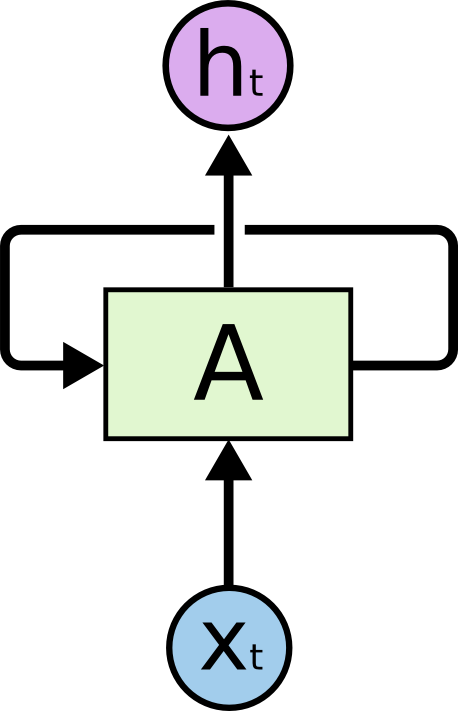
\includegraphics[scale=0.5]{RNN-rolled.png}
\end{figure}
上面的图表示一个RNN单元,A得到输入$x_t$和输出$h_t$,A允许信息被循环从一步到下一步,一个循环神经网络可以看成是多个相同单元的复制。铺开RNN可以得到
\begin{figure}[!ht]
\centering
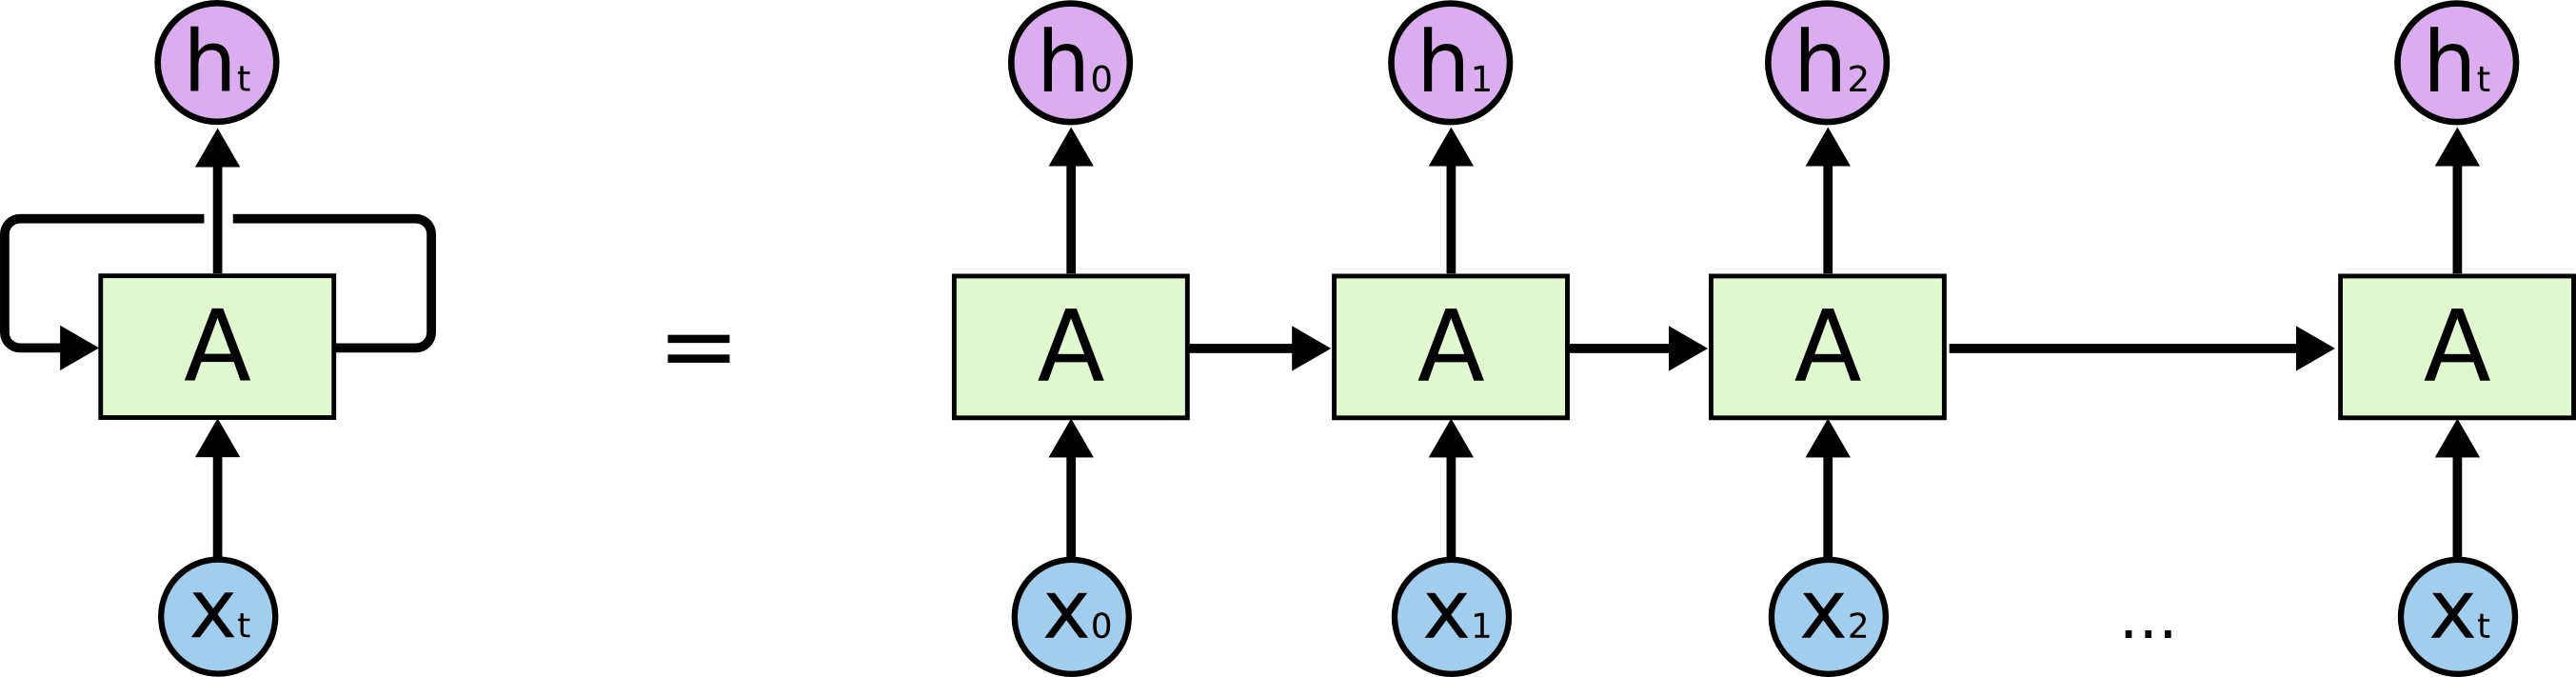
\includegraphics[scale=0.3]{RNN-unrolled.png}
\caption{unrolled RNN}
\end{figure}
这个链式结构揭示了循环神经网络和序列或者列表密切相关,它适用于这种数据。
\subsection{The Problem Long-Term Dependencies}
语言模型中常用先前的一个词预测下一个词,如果我们尝试预测"the clouds are in the {\color{red}{sky}}"我们不需要很多上下文信息RNN通过之前的信息就能学到。但是我们尝试预测这样一个句子"I grew up in France... I speak fluent {\color{red}{France}}",之前的信息暗示下一个单词可能是语言的名字,如果我们想去缩小语言的范围,我们需要上下文{\color{red}{France}},可相关信息和这个需要点的间隔很大。
\begin{figure}[!ht]
\centering
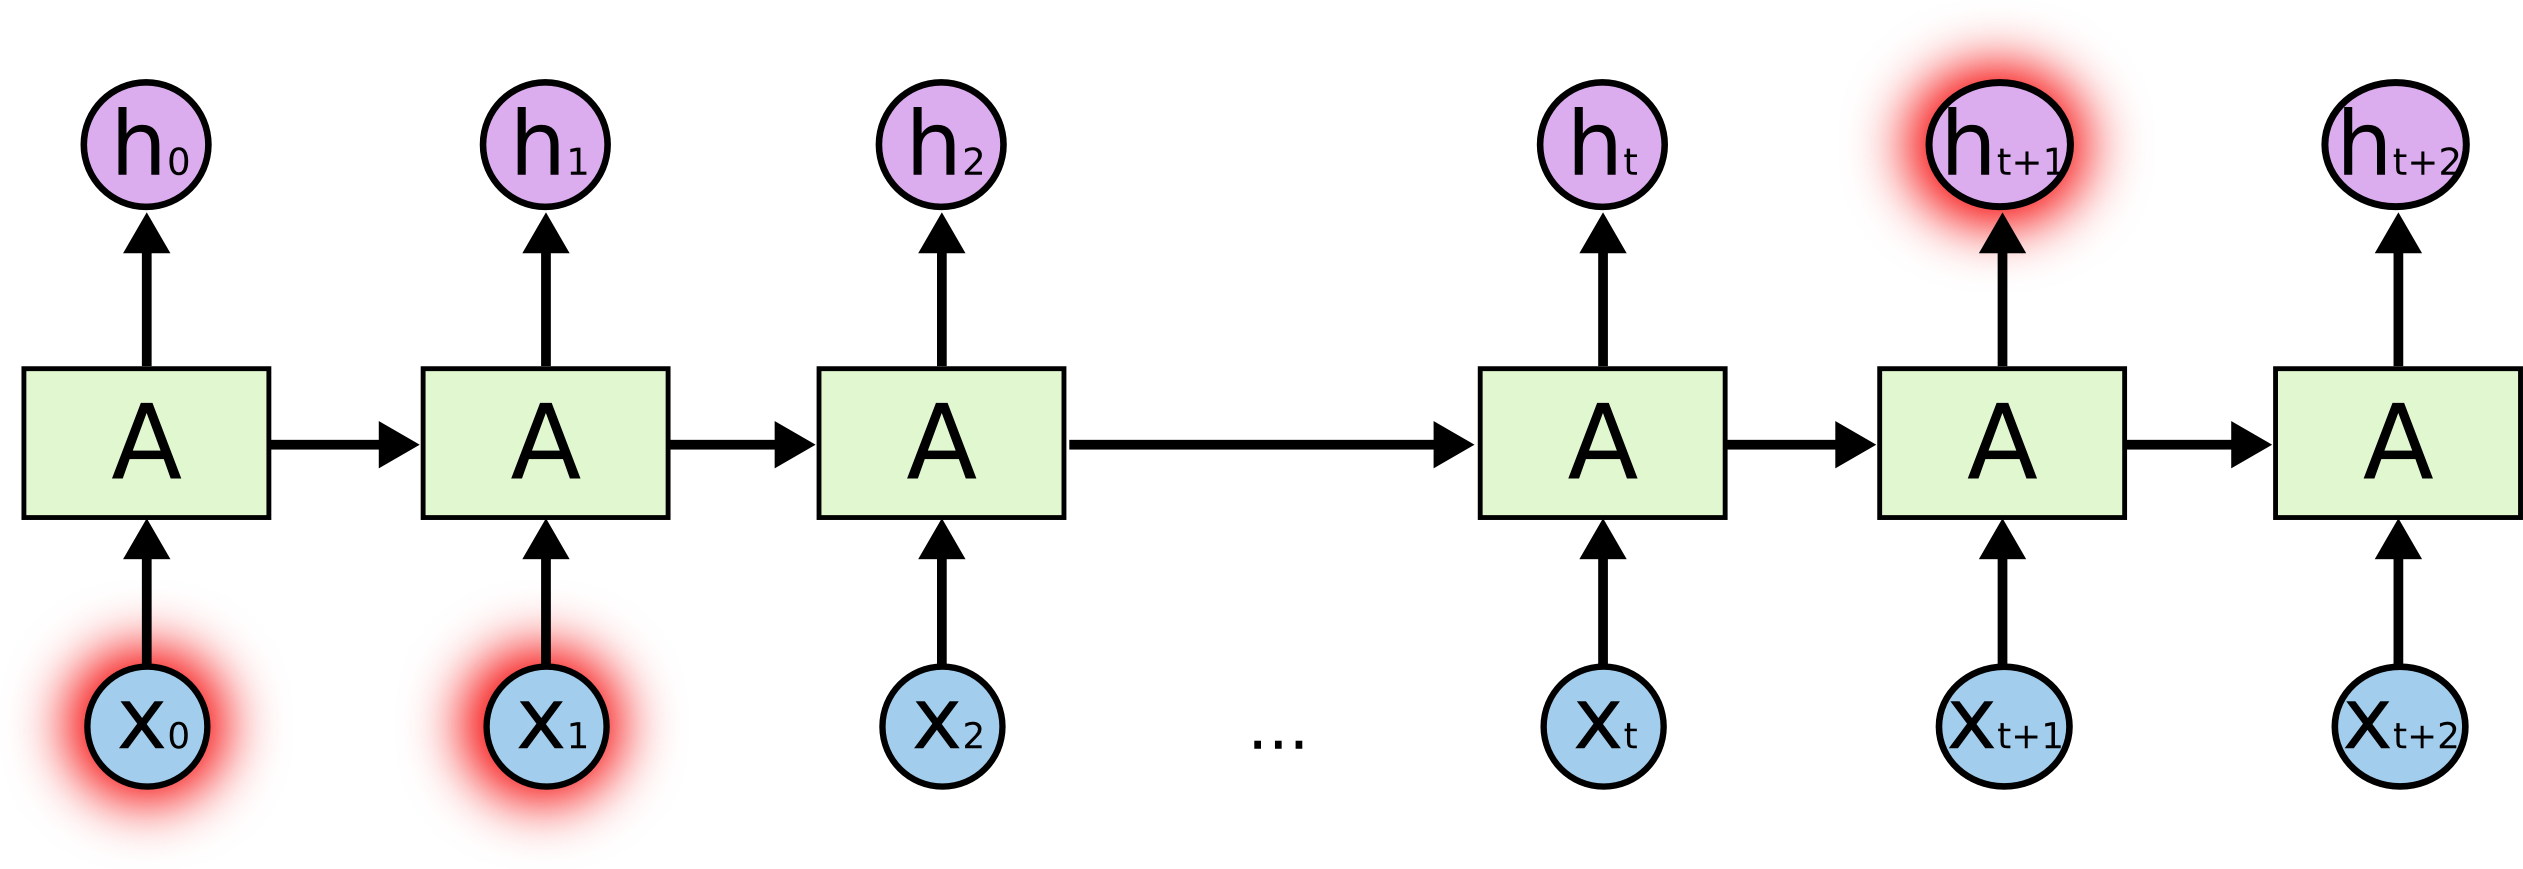
\includegraphics[scale=0.3]{RNN-longtermdependencies.png}
\end{figure}
理论上RNN有能力处理“long-term dependencies”,人能小心的挑选参数解决这个烦人的问题,然而不幸的是RNN似乎不能做到,原因由\href{http://www-dsi.ing.unifi.it/~paolo/ps/tnn-94-gradient.pdf}{Hochreiter (1991) [German] and Bengio, et al. (1994)}提出.
\subsection{LSTM网络}
Long Short Term Memory networks通常简称为LSTMs是一个特殊的RNN,能学习learning long-term dependencies,他被\href{http://deeplearning.cs.cmu.edu/pdfs/Hochreiter97_lstm.pdf}{Hochreiter  Schmidhuber (1997)}引入,然后被提炼,在大型文体处理上效果很好因而被广泛的使用。\par
LSTMs明确的设计去解决 long-term dependency problem。\par
所有的循环神经网络都有重复的链式形式。在标准的RNNs,重复的模块有一个非常简单的结构,像tanh Layer。
\begin{figure}
\centering
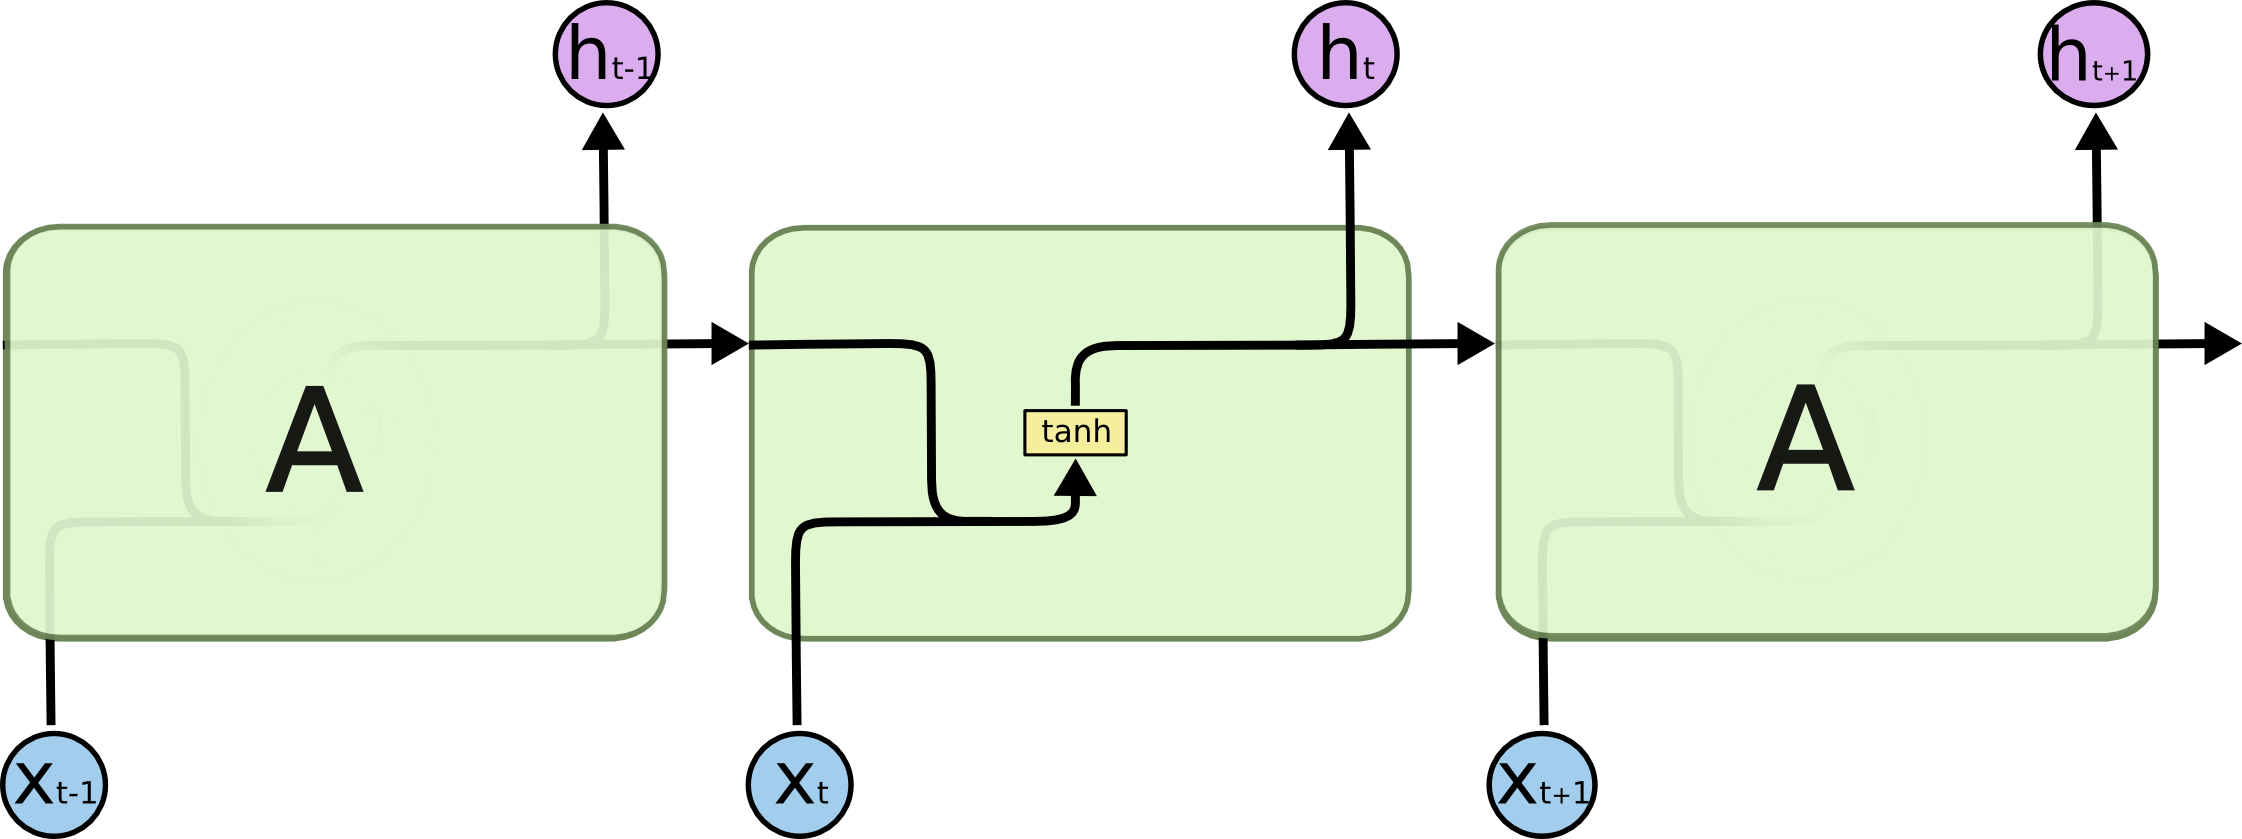
\includegraphics[scale=0.3]{LSTM3-SimpleRNN.png}
\caption{The repeating module in a standard RNN contains a single layer}
\end{figure}
LSTMs也有这样类似的结构,但是congruent模块有点不同,有一个神经网络层有四个相互作用部分,
\begin{figure}
\centering
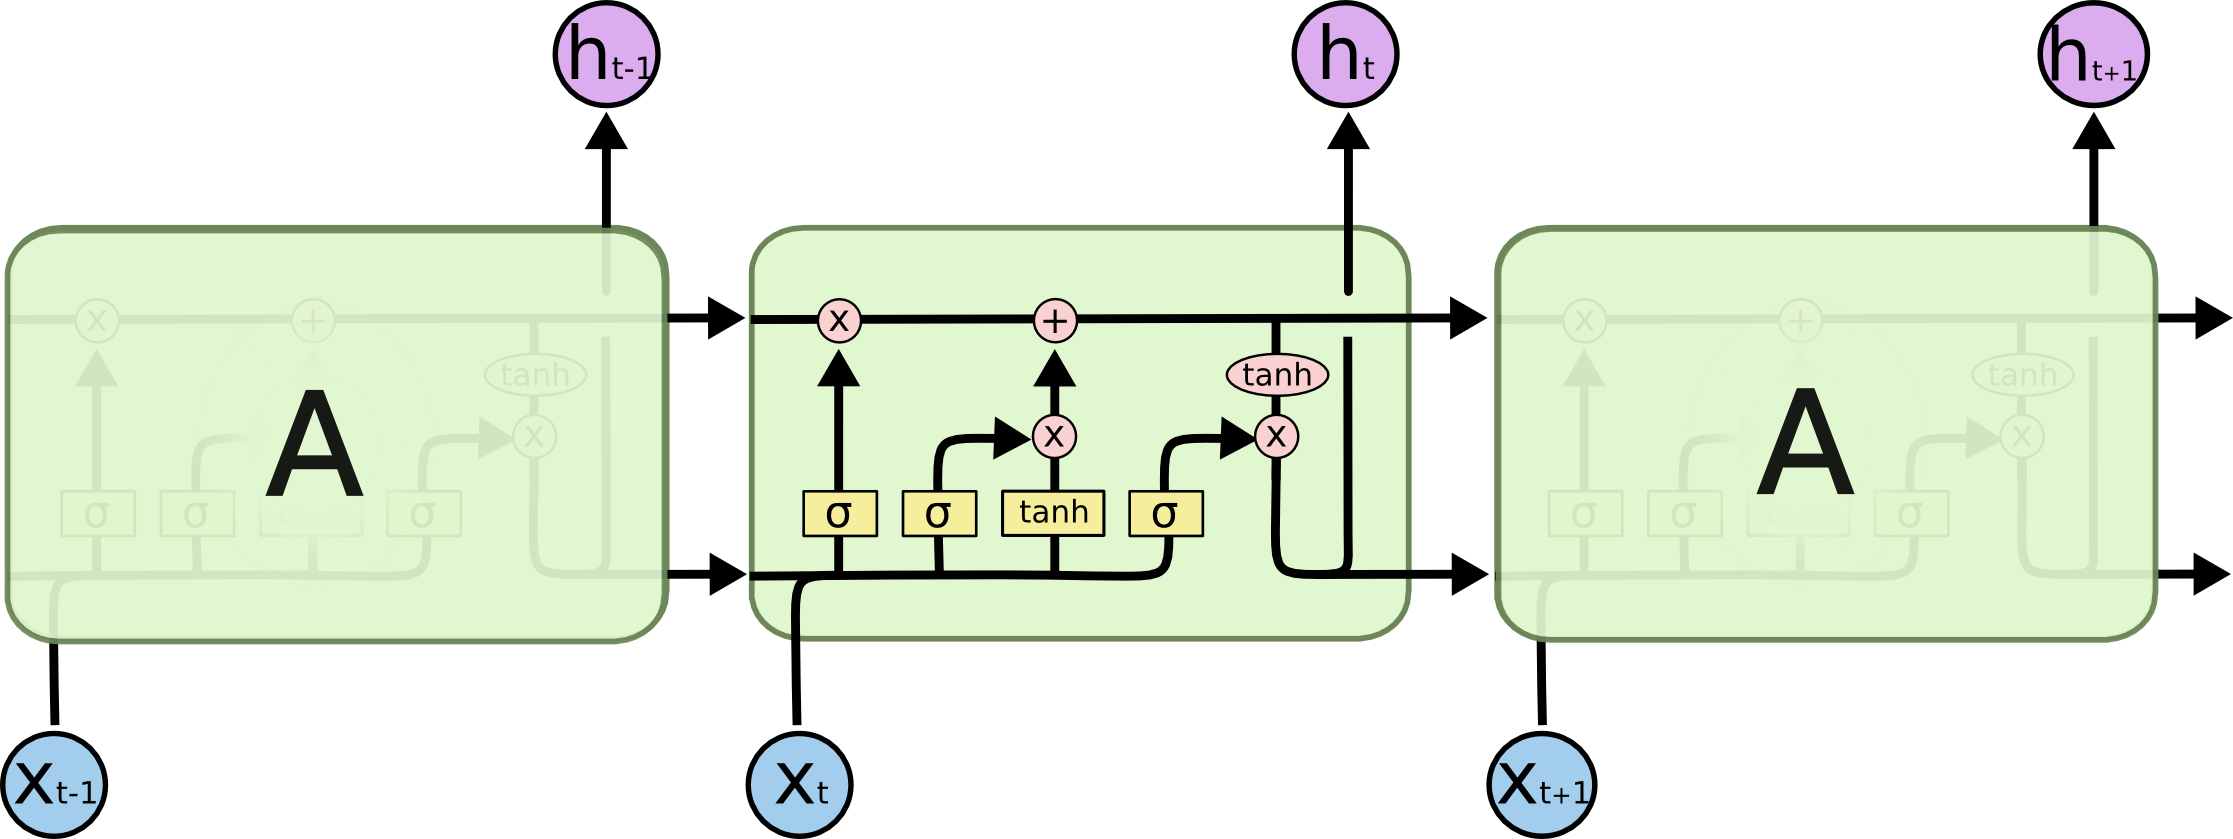
\includegraphics[scale=0.3]{LSTM3-chain.png}
\caption{The repeating module in an LSTM contains four interacting layers}
\end{figure}
\begin{figure}
\centering
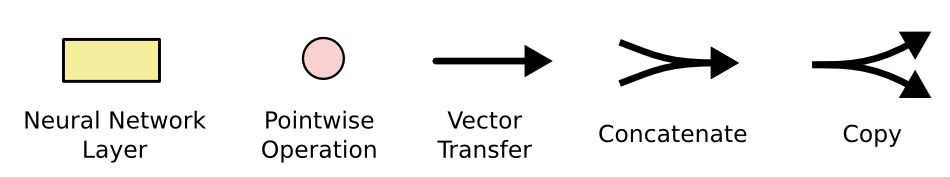
\includegraphics[scale=0.3]{LSTM2-notation.png}
\end{figure}
在上面的图上,每一根线上携带的都是一个向量,从一个输出节点到其他输入,粉色圆圈代表按点操作,黄色盒子是学习好的神经网络层,线融合表示串联,copy表示将一条线复制一份。
\subsection{LSTMs想法的核心}
LSTMs的核心是图像顶部的水平流过的cell state,cell state像一个传送带,它笔直的沿着整条链跑,和一些次要的线性交互,很容易实现信息不改变的流动。
\begin{figure}
\centering
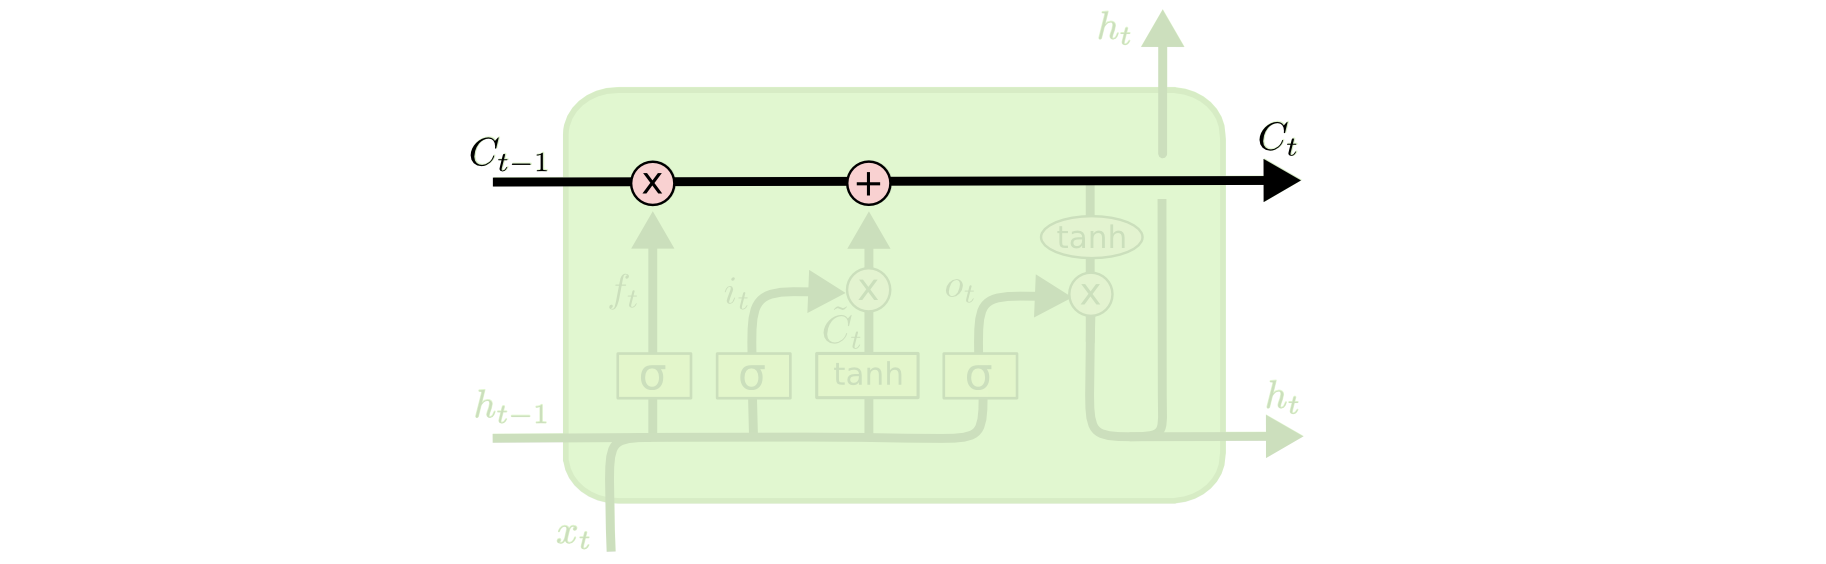
\includegraphics[scale=0.3]{LSTM3-C-line.png}
\end{figure}
LSTM能删除或者增加信息到cell state,被控制的结构称为门。门是一种让信息通过的手段,由一个sigmoid神经网络层和pointwise惩罚操作组成。
\begin{figure}
\centering
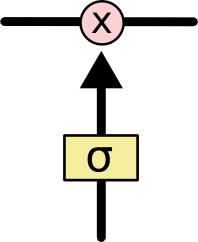
\includegraphics[scale=0.5]{LSTM3-gate.png}
\end{figure}
sigmod Layer输出0到1之间的数,描述多少组件应该被通过,0表示不允许通过1表示让一切通过,LSTMs有三个门,保护和控制cell state。
\subsection{一步步的设置}
第一步是LSTMs决定什么信息应该被传送,这个决定每一个称为忘记门的sigmoid layer组成,通过$h_{t-1}$和$x_t$输出0到1之间的数给当前的$C_{t-1}$,1表示完全保持,0表示丢弃。\par
对于上面的语言模型,cell state也许包含the gender of the present subjects,以至于正确的带名字能被使用,当我们看一个新的subject,我们想图忘记the gender of the old subject。
\begin{figure}
\centering
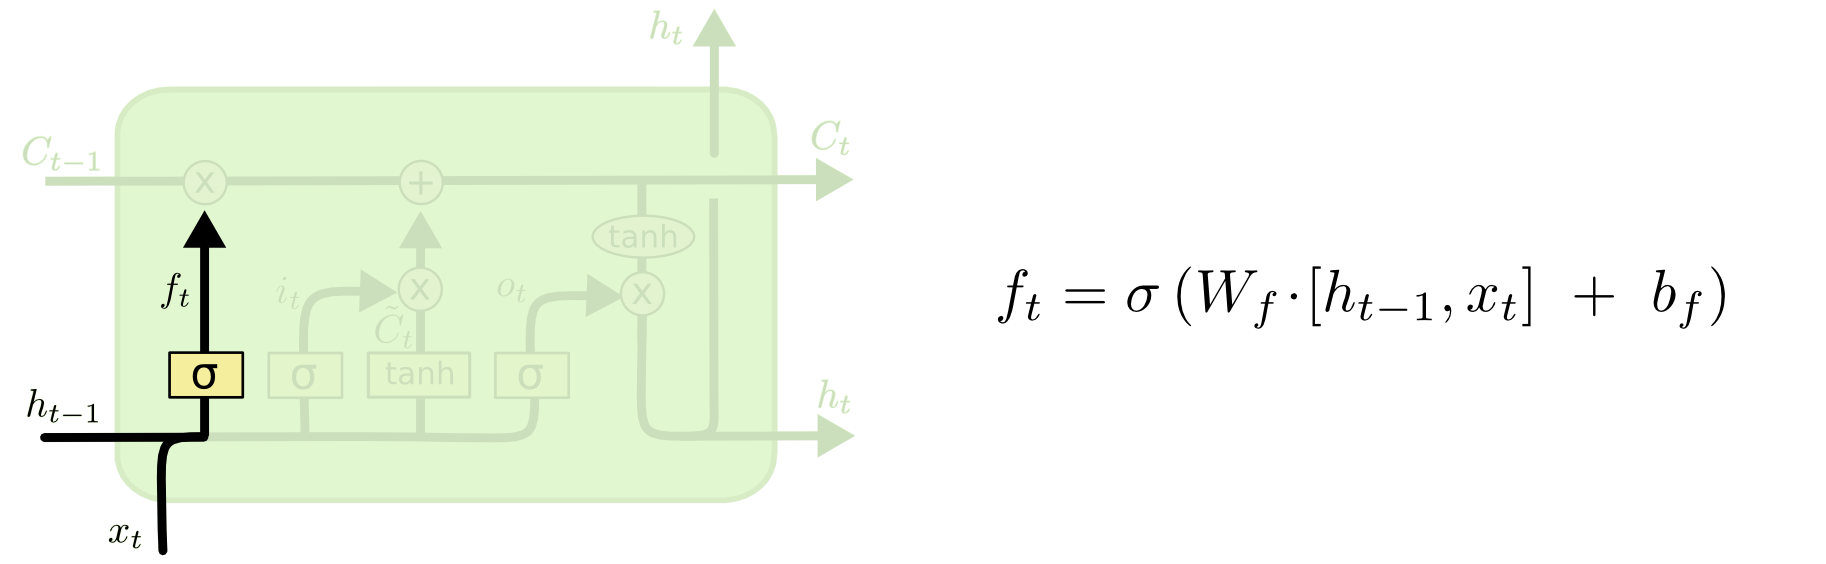
\includegraphics[scale=0.5]{LSTM3-focus-f.png}
\end{figure}
下一步是决定什么新的信息将被存储在cell state中,这分为两部分
\begin{enumerate}
	\item Sigmod layer调用 input gate layer决定更新哪个值。
	\item tanh layer创建一个可能被添加到state新的候选向量。$\widetilde{C_t}$
\end{enumerate}
下一步我们结合两个不走创建一个更新状态。,在我们的语言模型例子中,我们想要增加gender of the new subject到cell state取代我们将要忘记的数据
\begin{figure}
\centering
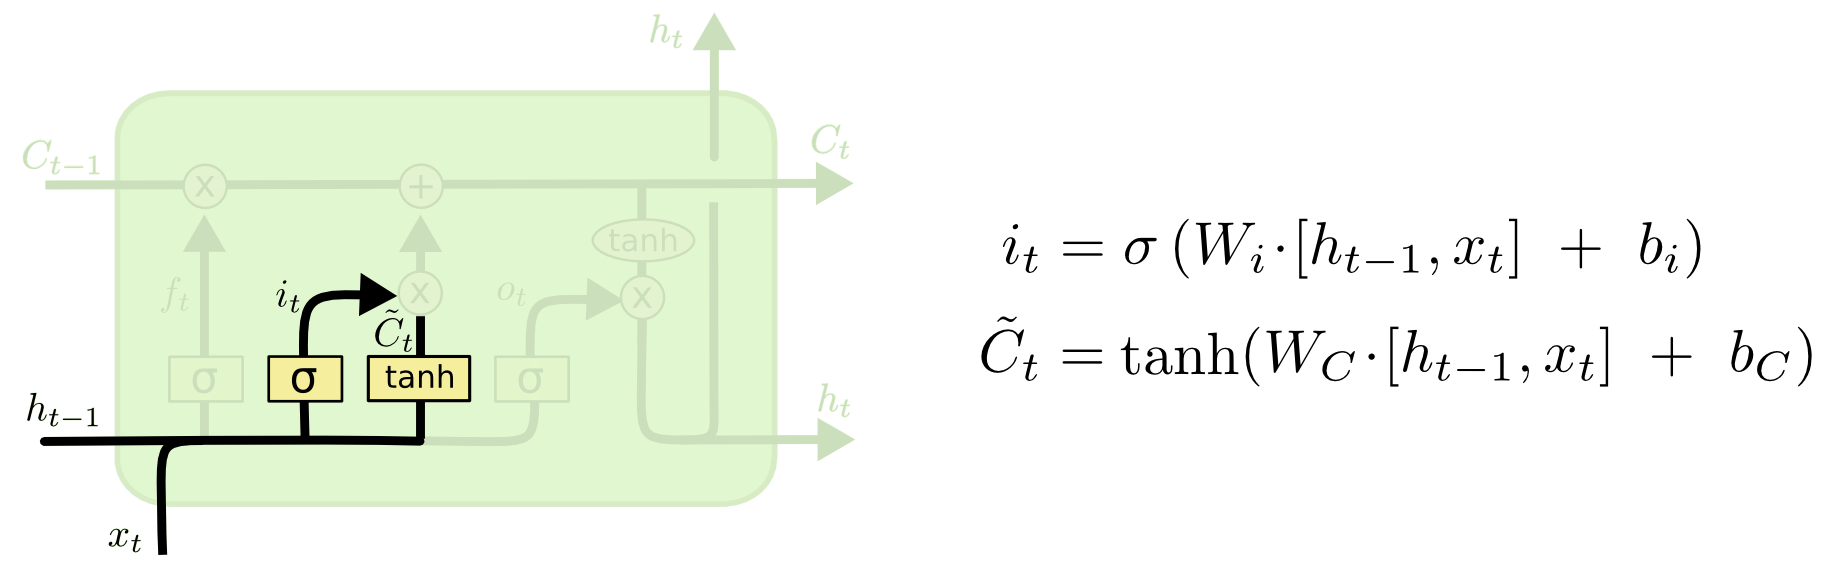
\includegraphics[scale=0.5]{LSTM3-focus-i.png}
\end{figure}
现在更新老的cell state$C_{t-1}$到新的cell state$C_t$,我们用老的$c_{t-1}$乘上$f_t$忘记我们之前决定忘记的事,然后我们增加$i_t*\widetilde{C_t}$.这是新的候选值,表示我们更新每个状态值的规模。在例子中的语言模型,我们删掉了一个老的subject's gender增加新的信息。
\begin{figure}
\centering
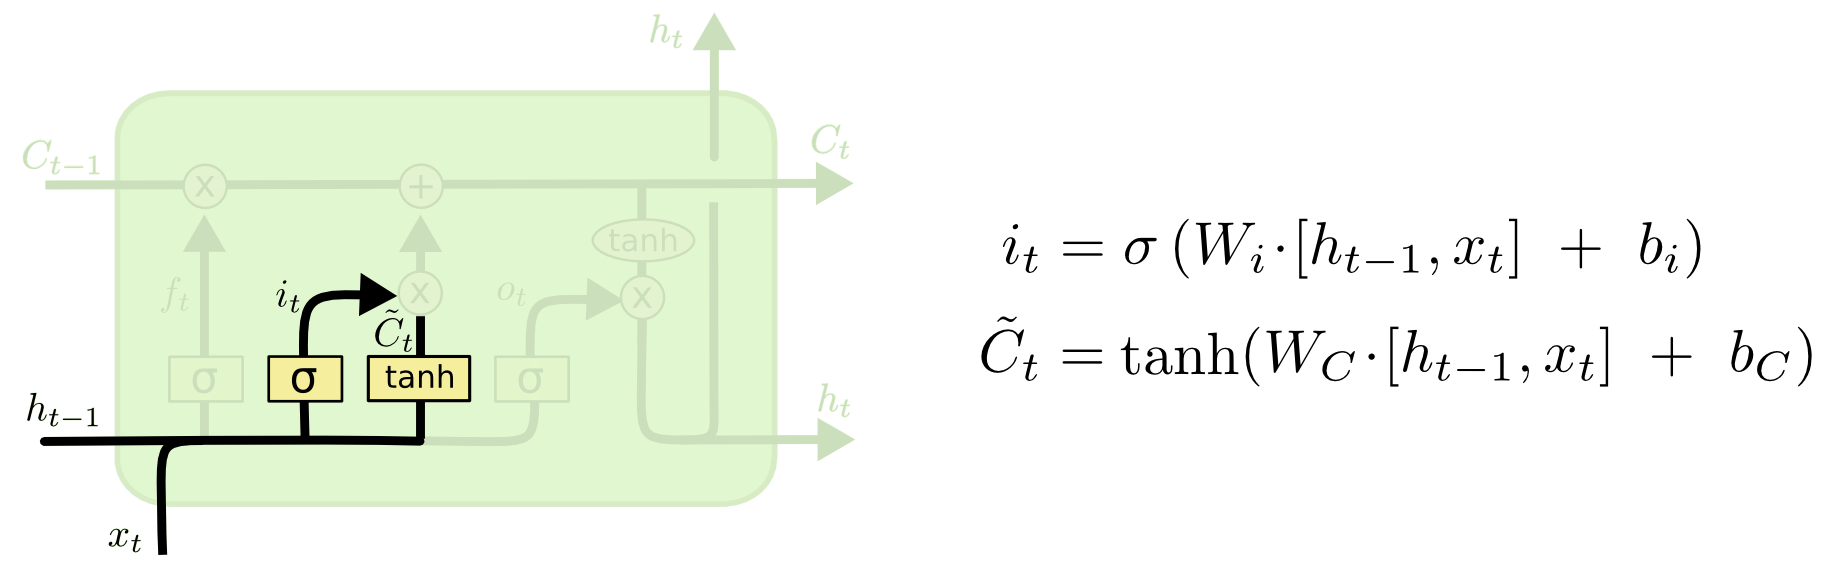
\includegraphics[scale=0.5]{LSTM3-focus-i.png}
\end{figure}
最后我们需要决定我们输出什么,输出取决于我们的cell state,但是将被过滤,所限我们运行sigmoid layer决定我们将输出那一部分。然后我们放通过tanh将cell state映射到-1,1,然后乘上sigmoid门的输出,以至于我们仅仅输出我们决定输出的部分。\par
对于语言模型的例子,因为它仅仅看subject,它也许想输出关于动词的信息,例子中的下一个,例如,它也许输出是否subject是单数或者复数,以至于从一个动词应该能知道接下来应该是动词的什么形式。
\begin{figure}
\centering
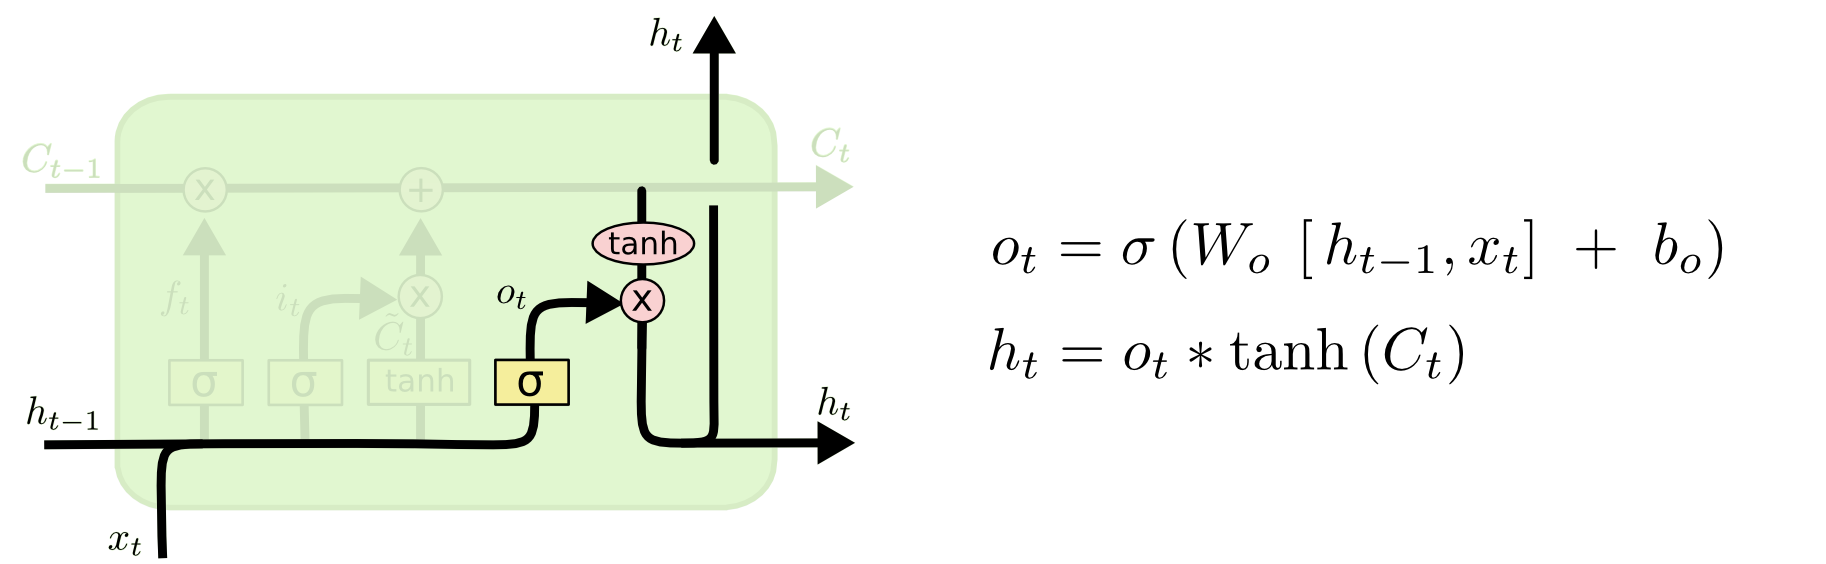
\includegraphics[scale=0.5]{LSTM3-focus-o.png}
\end{figure}
\subsection{LSTM的多种变体}
\href{ftp://ftp.idsia.ch/pub/juergen/TimeCount-IJCNN2000.pdf}{Gers  Schmidhuber (2000)},它增加了peephole connections,这一位置我们让gate layer通过cell state
\begin{figure}
\centering
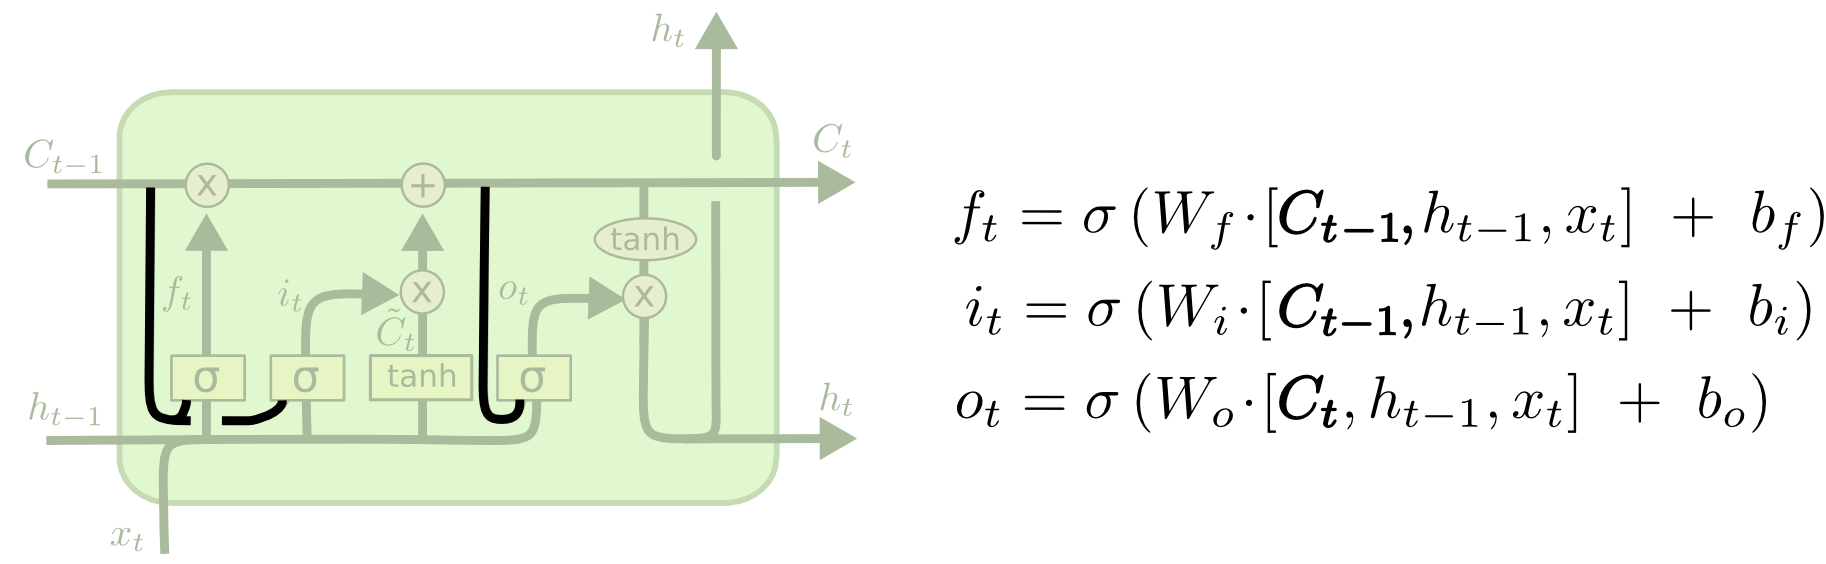
\includegraphics[scale=0.5]{LSTM3-var-peepholes.png}
\end{figure}
上面的图增加了peepholes到所有的门,但是一些论文给出一些peepholes和not others。另一个变体用两个forget 和输入门。而不是分别决定忘记或者添加信息,我们一起决定,我们需要输入一些值是忘记,我们仅仅忘记老的值输入新值到state
\begin{figure}
\centering
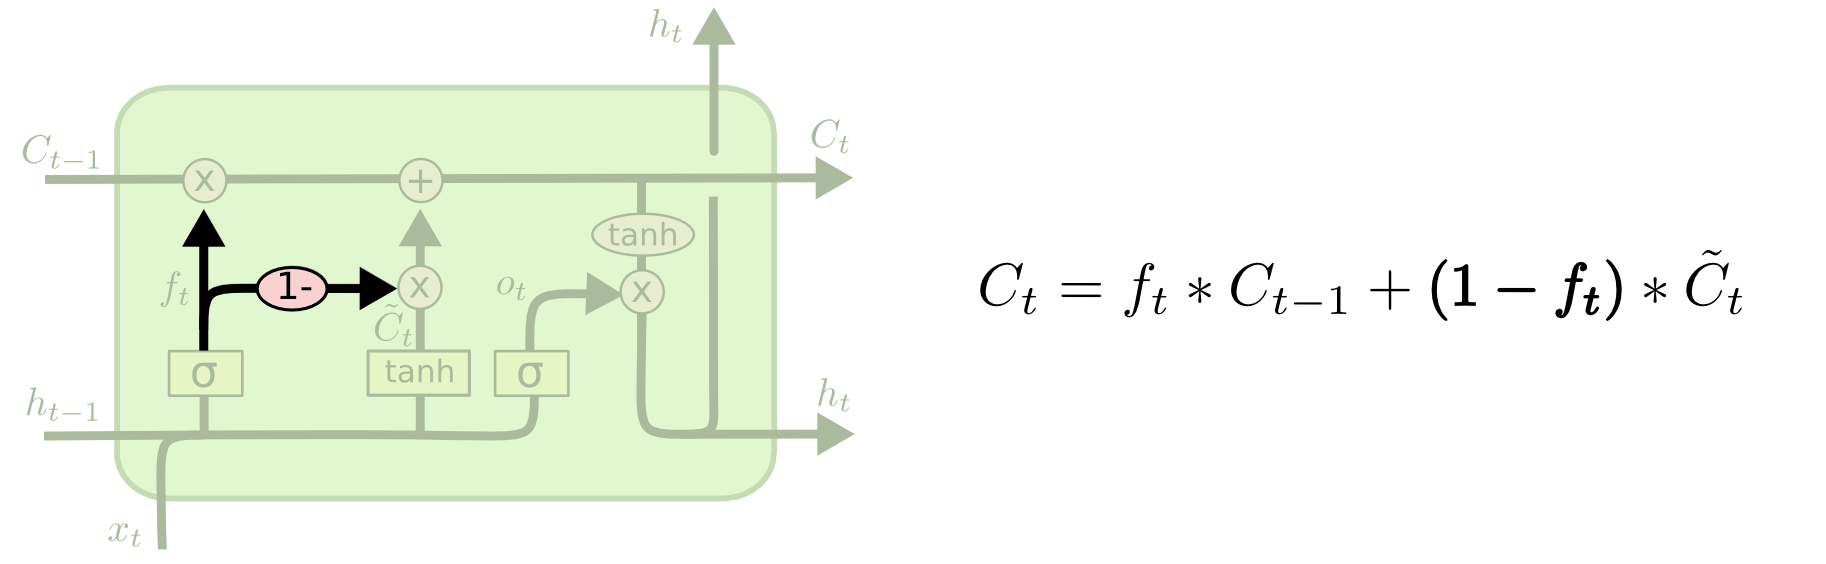
\includegraphics[scale=0.5]{LSTM3-var-tied.png}
\end{figure}
一个更引人注目的变体是Gate Recurrent Unit或者称为(GRU),由\href{http://arxiv.org/pdf/1406.1078v3.pdf}{Cho, et al. (2014)}引入,它结合忘记和输入门为一个单独的更新们,它也融合cell state和hidden state做了些改变,这结果模型比标准的LSTM模型简单,现在也越来越流行。
\begin{figure}
\centering
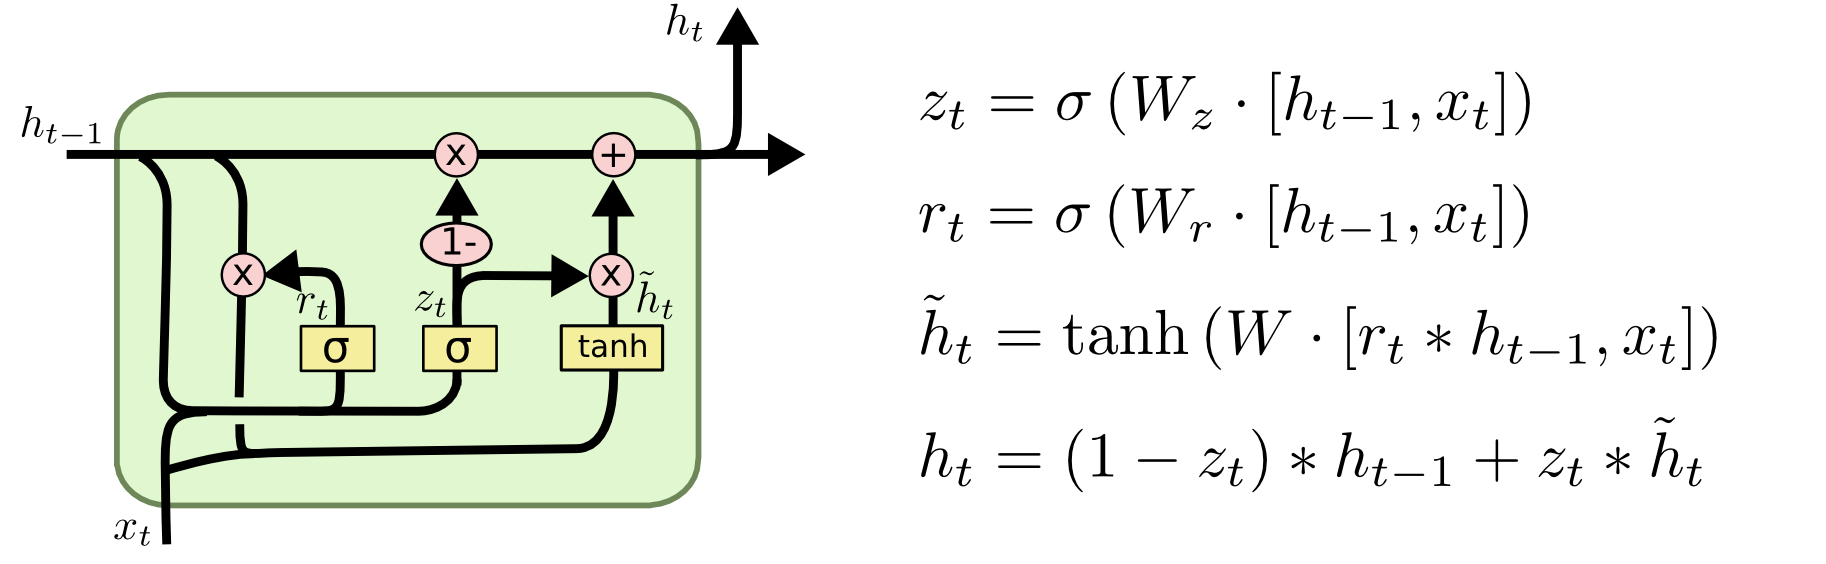
\includegraphics[scale=0.5]{LSTM3-var-GRU.png}
\end{figure}
这些仅仅是非常流行的LSTM变体,有一些其它的像\href{http://arxiv.org/pdf/1508.03790v2.pdf}{Yao, et al. (2015)}的Depth Gated RNNs,用完全不同的方法处理long-term dependencies,像\href{http://arxiv.org/pdf/1402.3511v1.pdf}{Koutnik, et al. (2014)}的Clockwork RNNs。\par
那个算法是最好的?他们的差别大吗?\href{http://arxiv.org/pdf/1503.04069.pdf}{Greff, et al. (2015) }做了一些比较了一些流行的变体,发现他们基本相同。
\href{http://jmlr.org/proceedings/papers/v37/jozefowicz15.pdf}{Jozefowicz, et al. (2015)}比较了超过1万中架构,找到了一些在确定问题上比LSTMs好的架构。
